% Partie devenir sponsor

Capitole du Libre recherche des partenaires financer l'événement et que l'évenment reste libre et accessible au plus grand nombre de personnes. Nous proposons à tout type d'entreprises de nous aider avec différents niveaux de sponsorins détaillés ci-dessous.

\Separateur

Nous sponsoriser, c'est vous associer à cette manifestation et contribuer au Logiciel Libre. Capitole du Libre est un lieu idéal pour venir découvrir de nouveaux horizons, récolter de nouvelles idées, découvrir de nouveaux talents

	\subsection{Niveaux de sponsoring}

    \begin{tabular}{|r|c|c|c|c|c|}
        \hline  & Bronze & Argent & Or & Platine & Diamant \\
        \hline Contribution & 250€ & 600€ & 1000€ & 2000€ & 3000€ \\
        \hline Limite & - & - & - & 4 & 2 \\
        \hline Logo sur l'affiche et le site web & \ding{'064} & \ding{'064} & \ding{'064} & \ding{'064} & \ding{'064}  \\
        \hline Badges sponsors & \ding{'064} & \ding{'064} & \ding{'064} & \ding{'064} & \ding{'064} \\
        \hline Dépôt d'offre d'emploi et de stage & \ding{'064} & \ding{'064} & \ding{'064} & \ding{'064} & \ding{'064} \\
        \hline Logo diffusé entre les conférences & & \ding{'064} & \ding{'064} & \ding{'064} & \ding{'064} \\
        \hline Logo au début de chaque video & & & \ding{'064} & \ding{'064} & \ding{'064} \\
        \hline Logo sur les flyers de l'événement & & & \ding{'064} & \ding{'064} & \ding{'064} \\
        \hline Texte sur le programme distribué & & & 1/4 page & 1/2 page & 1 page \\
        \hline Stand à proximité des buvettes & & & & 1 table & 2 tables \\
        \hline Remerciements lors de la conférence de clôture & & & & \ding{'064} & \ding{'064}  \\
        \hline Une idée? Contactez-nous! & & & & & \ding{'064} \\
        \hline Mise à disposition d'une salle privative & & & & & \ding{'064} \\
        \hline 
    \end{tabular}

Note: sur les différents supports, la taille de votre logo sera proportionnelle à votre niveau de support.

	\subsection{Retour d’expérience des précédents \textit{sponsors}}
	\subsection{Budget de l’événement}

Le budget total de l'édition 2014 de Capitole du Libre s'élevait à 12000€. Les différents postes de dépense sont indiqués dans le graphique ci-dessous:

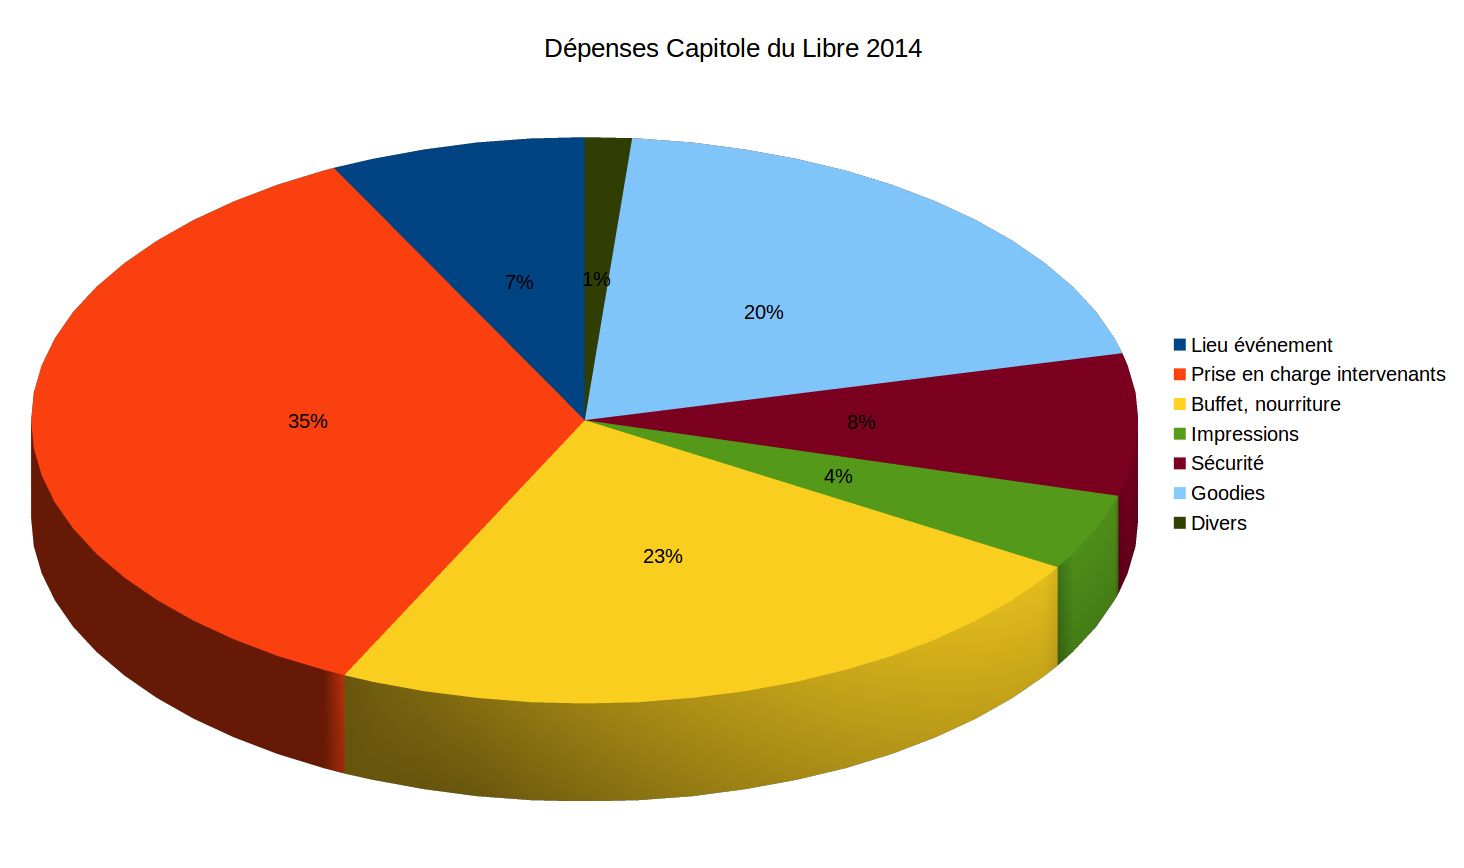
\includegraphics[scale=0.6]{Images/budget_2014.png}\\

Pour l'édition 2015 de Capitole du Libre, nous prévoyons une augmentation de notre budget à 18000 € afin principalement:
\begin{itemize}[label=$\bullet$]
\item de permettre de faire venir plus d'orateurs de plus loin afin de continuer à améliorer la qualité et la variété de nos orateurs
\item de réaliser un buffet correct le samedi soir (l'année dernière nous avions été vraiment trop juste en quantité). Ce buffet ouvert à tous et à participation libre étant un lieu d'échange privilégié lors de ce week-ends où se retrouvent orateur et particiapants des différentes thématiques.
\end{itemize}

\Separateur

Le détail des dépenses de Capitole du Libre 2015 est détaillé dans le tableau ci-dessous:

    \begin{tabular}{|l|c|}
        \hline Dépense & Montant \\
        \hline \textbf{Défraiements intervenants} & \textbf{5000 €} \\
        \hline Déplacements intervenants & 3500 € \\
        \hline Hébergement intervenants & 1500 € \\
        \hline \textbf{Hébergement manifestation} & \textbf{3000 €}\\
        \hline Chauffage & 1500 € \\
        \hline Sécurité & 1500 € \\
        \hline \textbf{Apéritif \& Repas} & \textbf{6000 € }\\
        \hline Participation repas intervenants et bénévoles & 1500 € \\
        \hline Buffet samedi soir & 4500 € \\
        \hline \textbf{Buvette} & \textbf{600€ }\\
        \hline Viénoiseries bénévoles & 150 € \\
        \hline Approvisionnement buvette & 400 € \\
        \hline Location machines à café & 50 € \\
        \hline \textbf{Goodies} & \textbf{2800 € }\\
        \hline T-Shirt Capitole du Libre 2015 & 1400 € \\
        \hline Goodies autres & 1400 € \\
        \hline \textbf{Communication} & \textbf{800 €} \\
        \hline Impression Flyyers & 100 € \\
        \hline Impression Affiches & 100 € \\
        \hline Impression Programmes & 500 € \\
        \hline Fléchage / Indications & 100 € \\
        \hline TOTAL & 18200 € \\
        \hline
    \end{tabular}

\Separateur

Les recettes 2015 sont détaillées dans le tableau ci-dessous:

    \begin{tabular}{|c|c|c|c|c|c|}
        \hline Dépense & Montant \\
        \hline Sponsors & 15 900 € \\
        \hline Dons & 300 € \\
        \hline Ventes buvette & 600 € \\
        \hline Recette boutique & 1600 € \\
        \hline TOTAL & 18200 € \\
        \hline
    \end{tabular}

